\documentclass{article}

% content/resources/templates/preamble.tex
\usepackage[margin=0.6in]{geometry}
\author{Milav Dabgar}
\usepackage{amsmath,amssymb,amsthm}
\usepackage{booktabs}
\usepackage{multirow}
\usepackage{xcolor}
\usepackage{tcolorbox}
\tcbuselibrary{breakable,skins}
\usepackage[colorlinks=true,linkcolor=blue]{hyperref}
\usepackage{titlesec}
\usepackage{enumitem}
\usepackage{tikz}
\usepackage{pgfplots}
\usepackage{circuitikz}
\usepackage[version=4]{mhchem}
\usepackage{longtable}
\usepackage{array}
\usepackage{float}
\usepackage{caption}
\usepackage{listings}

\lstset{
  basicstyle=\small\ttfamily,
  breaklines=true,
  breakatwhitespace=false,
  postbreak=\mbox{\textcolor{red}{$\hookrightarrow$}\space},
  float=false,
  numbers=left,
  numberstyle=\tiny\color{gray},
  numbersep=10pt,
  xleftmargin=2em,
  keywordstyle=\color{blue},
  commentstyle=\color{green!60!black},
  stringstyle=\color{purple},
  backgroundcolor=\color{gray!5},
  showstringspaces=false,
  tabsize=2,
  captionpos=b,
  keepspaces=true,
  columns=flexible
}

\pgfplotsset{compat=1.18}
\usetikzlibrary{shapes,arrows,positioning,calc,patterns,decorations.pathmorphing,decorations.markings,arrows.meta}

% Color scheme
\definecolor{headcolor}{RGB}{0,102,204}
\definecolor{keycolor}{RGB}{220,20,60}
\definecolor{solutioncolor}{RGB}{34,139,34}
\definecolor{mnemoniccolor}{RGB}{148,0,211}
\definecolor{codecolor}{RGB}{0,0,100}

% Spacing
\setlength{\parskip}{3pt}
\setlist[itemize]{nosep}
\setlist[enumerate]{nosep}

% Title formatting
\titleformat{\section}{\Large\bfseries\color{headcolor}}{\thesection}{1em}{}
\titleformat{\subsection}{\large\bfseries\color{headcolor}}{\thesubsection}{1em}{}

% Pandoc tightlist compatibility
\providecommand{\tightlist}{%
  \setlength{\itemsep}{0pt}\setlength{\parskip}{0pt}}

% Pandoc longtable compatibility
\newcounter{none}
\def\thenone{}


% content/resources/templates/english-boxes.tex

% Custom environments
\newtcolorbox{solutionbox}{
 breakable,
 enhanced,
 colback=solutioncolor!5!white,
 colframe=solutioncolor!75!black,
 fonttitle=\bfseries,
 title=Solution
}

\newtcolorbox{solutionboxnobreak}{
 colback=solutioncolor!5!white,
 colframe=solutioncolor!75!black,
 fonttitle=\bfseries,
 title=Solution
}

\newtcolorbox{keyformula}{
 breakable,
 enhanced,
 colback=keycolor!5!white,
 colframe=keycolor!75!black,
 fonttitle=\bfseries,
 title=Key Formula
}

\newtcolorbox{mnemonicboxenv}{
 breakable,
 enhanced,
 colback=mnemoniccolor!5!white,
 colframe=mnemoniccolor!75!black,
 fonttitle=\bfseries,
 title=Mnemonic
}

\newcommand{\mnemonicbox}[1]{%
  \begin{mnemonicboxenv}
    #1
  \end{mnemonicboxenv}
}


% Custom commands for GTU solutions
% This file defines semantic commands for consistent formatting

% Question command with automatic formatting
\newcommand{\question}[2]{%
  \section*{Question #1}%
  \textbf{#2}%
}

% OR question variant
\newcommand{\questionor}[2]{%
  \section*{Question #1 OR}%
  \textbf{#2}%
}

% Proper table environment with caption
\newenvironment{answertable}[1]{%
  \begin{table}[htbp]
  \centering
  \caption{#1}
}{%
  \end{table}
}

% Proper figure environment for diagrams
\newenvironment{answerdiagram}[1]{%
  \begin{figure}[htbp]
  \centering
  \caption{#1}
}{%
  \end{figure}
}

% Semantic markup for key terms
\newcommand{\keyword}[1]{\textbf{#1}}
\newcommand{\code}[1]{\texttt{#1}}
\newcommand{\classname}[1]{\texttt{#1}}
\newcommand{\methodname}[1]{\texttt{#1}}

% Proper quotation marks
\newcommand{\mnemonic}[1]{``#1''}


\title{Foundation of Blockchain (4361603) - Summer 2025 Solution}
\date{May 14, 2025}

\begin{document}
\maketitle

\questionmarks{1(a)}{3}{Differentiate between Private key and Public key in Blockchain.}

\begin{tabulary}{\linewidth}{L L L}
    \toprule
    \textbf{Aspect} & \textbf{Private Key} & \textbf{Public Key} \\
    \midrule
    \textbf{Purpose} & Used for signing transactions & Used for verification \\
    \textbf{Sharing} & Must be kept secret & Can be shared publicly \\
    \textbf{Function} & Decrypts data, creates signatures & Encrypts data, verifies signatures \\
    \textbf{Ownership} & Only owner knows it & Everyone can access it \\
    \bottomrule
\end{tabulary}

\begin{itemize}
    \item \keyword{Private Key}: Secret mathematical code that proves ownership
    \item \keyword{Public Key}: Open address that others use to send transactions
    \item \keyword{Security}: Private key loss = permanent fund loss
\end{itemize}

\begin{mnemonicbox}
Private is Personal, Public is Posted
\end{mnemonicbox}

\questionmarks{1(b)}{4}{Explain Distributed Ledger in detail.}

\textbf{Distributed Ledger} is a database spread across multiple locations and participants.

\begin{tabulary}{\linewidth}{L L}
    \toprule
    \textbf{Feature} & \textbf{Description} \\
    \midrule
    \textbf{Decentralized} & No single control point \\
    \textbf{Synchronized} & All copies stay updated \\
    \textbf{Transparent} & All participants can view \\
    \textbf{Immutable} & Cannot be easily changed \\
    \bottomrule
\end{tabulary}

\begin{figure}[H]
    \centering
    \begin{tikzpicture}[node distance=2cm, auto]
        \node [gtu block] (DL) {Distributed Ledger};
        \node [gtu block, above=of DL] (P2) {Participant 2};
        \node [gtu block, left=of P2] (P1) {Participant 1};
        \node [gtu block, right=of P2] (P3) {Participant 3};
        \node [gtu block, below=of DL] (SC2) {Synchronized Copy 2};
        \node [gtu block, left=of SC2] (SC1) {Synchronized Copy 1};
        \node [gtu block, right=of SC2] (SC3) {Synchronized Copy 3};

        \draw [gtu arrow] (P1) -- (DL);
        \draw [gtu arrow] (P2) -- (DL);
        \draw [gtu arrow] (P3) -- (DL);
        \draw [gtu arrow] (DL) -- (SC1);
        \draw [gtu arrow] (DL) -- (SC2);
        \draw [gtu arrow] (DL) -- (SC3);
    \end{tikzpicture}
    \caption{Distributed Ledger System}
\end{figure}

\begin{itemize}
    \item \keyword{Benefits}: Eliminates intermediaries, increases trust, reduces fraud
    \item \keyword{Working}: All participants maintain identical copies of records
\end{itemize}

\begin{mnemonicbox}
Distributed = Divided but Identical
\end{mnemonicbox}

\questionmarks{1(c)}{7}{Define Blockchain. Describe applications and limits of Blockchain.}

\keyword{Blockchain Definition}: A chain of blocks containing transaction records, linked using cryptography.

\textbf{Applications:}

\begin{tabulary}{\linewidth}{L L L}
    \toprule
    \textbf{Sector} & \textbf{Application} & \textbf{Benefit} \\
    \midrule
    \textbf{Finance} & Cryptocurrency, payments & Faster, cheaper transfers \\
    \textbf{Healthcare} & Patient records & Secure, accessible data \\
    \textbf{Supply Chain} & Product tracking & Transparency, authenticity \\
    \textbf{Real Estate} & Property records & Fraud prevention \\
    \textbf{Voting} & Digital elections & Transparent, tamper-proof \\
    \bottomrule
\end{tabulary}

\textbf{Limits:}

\begin{tabulary}{\linewidth}{L L}
    \toprule
    \textbf{Limitation} & \textbf{Impact} \\
    \midrule
    \textbf{Scalability} & Slow transaction processing \\
    \textbf{Energy Usage} & High electricity consumption \\
    \textbf{Complexity} & Difficult for users to understand \\
    \textbf{Regulation} & Legal uncertainty \\
    \textbf{Storage} & Growing data size problems \\
    \bottomrule
\end{tabulary}

\begin{figure}[H]
    \centering
    \begin{tikzpicture}[node distance=1.5cm, auto]
        \node [gtu block] (B1) {Block 1};
        \node [gtu block, right=of B1] (B2) {Block 2};
        \node [gtu block, right=of B2] (B3) {Block 3};
        \node [gtu block, right=of B3] (B4) {Block 4};

        \node [gtu state, below=0.5cm of B1] (H1) {Hash};
        \node [gtu state, below=0.5cm of B2] (H2) {Hash};
        \node [gtu state, below=0.5cm of B3] (H3) {Hash};
        \node [gtu state, below=0.5cm of B4] (H4) {Hash};

        \draw [gtu arrow] (B1) -- (B2);
        \draw [gtu arrow] (B2) -- (B3);
        \draw [gtu arrow] (B3) -- (B4);
        
        \draw [gtu arrow] (H1) -- (B1);
        \draw [gtu arrow] (H2) -- (B2);
        \draw [gtu arrow] (H3) -- (B3);
        \draw [gtu arrow] (H4) -- (B4);
    \end{tikzpicture}
    \caption{Blockchain Architecture}
\end{figure}

\begin{itemize}
    \item \keyword{Security}: Cryptographic linking makes tampering difficult
    \item \keyword{Transparency}: All transactions visible to network participants
\end{itemize}

\begin{mnemonicbox}
Blocks Chained = Blockchain, Apps Many = Limits Many
\end{mnemonicbox}

\orquestionmarks{1(c)}{7}{Write a short note on: CAP Theorem in Blockchain}

\keyword{CAP Theorem} states that distributed systems can only guarantee 2 out of 3 properties simultaneously.

\begin{tabulary}{\linewidth}{L L L}
    \toprule
    \textbf{Property} & \textbf{Description} & \textbf{Example} \\
    \midrule
    \textbf{Consistency} & All nodes have same data & Same balance shown everywhere \\
    \textbf{Availability} & System always responds & Network never goes down \\
    \textbf{Partition Tolerance} & Works despite network failures & Functions even if nodes disconnect \\
    \bottomrule
\end{tabulary}

\begin{figure}[H]
    \centering
    \begin{tikzpicture}[node distance=1.5cm, auto]
        \node [gtu block] (CAP) {CAP Theorem};
        \node [gtu state, below left=of CAP] (C) {Consistency};
        \node [gtu state, below=of CAP] (A) {Availability};
        \node [gtu state, below right=of CAP] (P) {Partition Tolerance};

        \node [gtu block, below=2cm of C] (BTC) {Bitcoin};
        \node [gtu block, below=2cm of P] (PVT) {Private Blockchain};

        \draw [gtu arrow] (CAP) -- (C);
        \draw [gtu arrow] (CAP) -- (A);
        \draw [gtu arrow] (CAP) -- (P);

        \draw [gtu arrow] (BTC) -- (C);
        \draw [gtu arrow] (BTC) -- (P);
        \draw [gtu arrow] (PVT) -- (C);
        \draw [gtu arrow] (PVT) -- (A);
    \end{tikzpicture}
    \caption{CAP Theorem and Blockchain Trade-offs}
\end{figure}

\textbf{Real-world Applications:}

\begin{tabulary}{\linewidth}{L L L}
    \toprule
    \textbf{Blockchain Type} & \textbf{Chooses} & \textbf{Sacrifices} \\
    \midrule
    \textbf{Bitcoin} & Consistency + Partition & Availability \\
    \textbf{Ethereum} & Consistency + Partition & Availability \\
    \textbf{Private Networks} & Consistency + Availability & Partition Tolerance \\
    \bottomrule
\end{tabulary}

\begin{itemize}
    \item \keyword{Impact}: Blockchain designers must choose which property to sacrifice
    \item \keyword{Trade-off}: Perfect systems impossible in distributed networks
\end{itemize}

\begin{mnemonicbox}
Can't Always Please - Choose 2 of 3
\end{mnemonicbox}

\questionmarks{2(a)}{3}{Explain Data Structure of a Blockchain.}

\textbf{Blockchain Data Structure} consists of linked blocks containing transaction data.

\begin{tabulary}{\linewidth}{L L}
    \toprule
    \textbf{Component} & \textbf{Purpose} \\
    \midrule
    \textbf{Block Header} & Contains metadata \\
    \textbf{Previous Hash} & Links to previous block \\
    \textbf{Merkle Root} & Summary of all transactions \\
    \textbf{Timestamp} & When block was created \\
    \textbf{Transactions} & Actual data/transfers \\
    \bottomrule
\end{tabulary}

\begin{figure}[H]
    \centering
    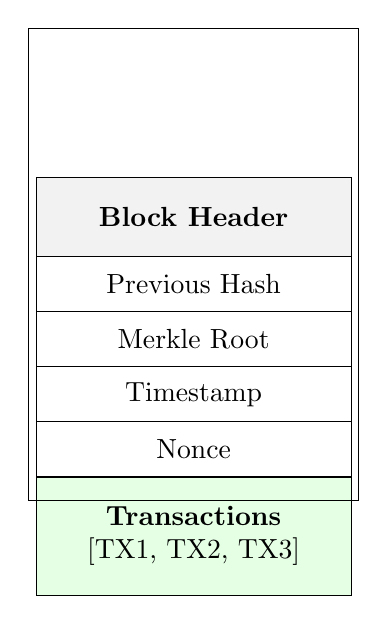
\begin{tikzpicture}[node distance=0cm, outer sep=0pt]
        \node [draw, rectangle, minimum width=4cm, minimum height=1cm, fill=gray!10] (Head) {\textbf{Block Header}};
        \node [draw, rectangle, minimum width=4cm, minimum height=0.7cm, below=0pt of Head] (Prev) {Previous Hash};
        \node [draw, rectangle, minimum width=4cm, minimum height=0.7cm, below=0pt of Prev] (Merkle) {Merkle Root};
        \node [draw, rectangle, minimum width=4cm, minimum height=0.7cm, below=0pt of Merkle] (Time) {Timestamp};
        \node [draw, rectangle, minimum width=4cm, minimum height=0.7cm, below=0pt of Time] (Nonce) {Nonce};
        \node [draw, rectangle, minimum width=4cm, minimum height=1.5cm, below=0pt of Nonce, fill=green!10, align=center] (Tx) {\textbf{Transactions}\\ {[TX1, TX2, TX3]}};
        
        \node [draw, rectangle, minimum width=4.2cm, minimum height=6cm, below=0pt of Head, yshift=2.9cm] (Block) {};
    \end{tikzpicture}
    \caption{Structure of a Block}
\end{figure}

\begin{itemize}
    \item \keyword{Linking}: Each block points to previous block using hash
    \item \keyword{Integrity}: Changing one block breaks the entire chain
\end{itemize}

\begin{mnemonicbox}
Header Holds, Transactions Tell
\end{mnemonicbox}

\questionmarks{2(b)}{4}{What are the benefits of Decentralization?}

\textbf{Decentralization Benefits:}

\begin{tabulary}{\linewidth}{L L}
    \toprule
    \textbf{Benefit} & \textbf{Explanation} \\
    \midrule
    \textbf{No Single Point of Failure} & Network continues if one node fails \\
    \textbf{Censorship Resistance} & No authority can block transactions \\
    \textbf{Transparency} & All participants see same information \\
    \textbf{Reduced Costs} & Eliminates intermediary fees \\
    \textbf{Trust} & No need to trust central authority \\
    \bottomrule
\end{tabulary}

\begin{figure}[H]
    \centering
    \begin{tikzpicture}[node distance=1.5cm]
        % Centralized
        \node [gtu state] (C) {Central};
        \node [gtu block, below left=of C] (U1) {User 1};
        \node [gtu block, below=of C] (U2) {User 2};
        \node [gtu block, below right=of C] (U3) {User 3};
        
        \draw [gtu arrow] (C) -- (U1);
        \draw [gtu arrow] (C) -- (U2);
        \draw [gtu arrow] (C) -- (U3);
        
        \node [below=0.5cm of U2] {Centralized};

        % Decentralized - shifted right
        \node [gtu block, right=5cm of U1] (D1) {User 1};
        \node [gtu block, right=of D1] (D2) {User 2};
        \node [gtu block, right=of D2] (D3) {User 3};
        
        \draw [gtu arrow, <->] (D1) -- (D2);
        \draw [gtu arrow, <->] (D2) -- (D3);
        \draw [gtu arrow, <->, bend left=45] (D1) to (D3);
        
        \node [below=0.5cm of D2] {Decentralized};
    \end{tikzpicture}
    \caption{Centralized vs. Decentralized Networks}
\end{figure}

\begin{itemize}
    \item \keyword{Security}: Multiple copies prevent data loss
    \item \keyword{Democracy}: All participants have equal rights
    \item \keyword{Resilience}: System survives individual failures
\end{itemize}

\begin{mnemonicbox}
Distributed = Durable, Democratic, Direct
\end{mnemonicbox}

\questionmarks{2(c)}{7}{Differentiate between Public Blockchain and Private Blockchain.}

\keyword{Comprehensive Comparison}:

\begin{tabulary}{\linewidth}{L L L}
    \toprule
    \textbf{Aspect} & \textbf{Public Blockchain} & \textbf{Private Blockchain} \\
    \midrule
    \textbf{Access} & Open to everyone & Restricted to specific users \\
    \textbf{Permission} & Permissionless & Requires permission \\
    \textbf{Control} & Decentralized & Centralized control \\
    \textbf{Speed} & Slower (consensus needed) & Faster (fewer validators) \\
    \textbf{Security} & High (many validators) & Medium (fewer validators) \\
    \textbf{Cost} & Transaction fees required & Lower operational costs \\
    \textbf{Transparency} & Fully transparent & Limited transparency \\
    \textbf{Examples} & Bitcoin, Ethereum & Hyperledger, R3 Corda \\
    \bottomrule
\end{tabulary}

\begin{figure}[H]
    \centering
    \begin{tikzpicture}[node distance=1.5cm]
        % Public
        \node [gtu block] (PubNet) {Global Network};
        \node [gtu state, above left=of PubNet] (Any1) {Anyone};
        \node [gtu state, above=of PubNet] (Any2) {Anyone};
        \node [gtu state, above right=of PubNet] (Any3) {Anyone};
        
        \draw [gtu arrow] (Any1) -- (PubNet);
        \draw [gtu arrow] (Any2) -- (PubNet);
        \draw [gtu arrow] (Any3) -- (PubNet);
        
        \node [below=0.2cm of PubNet] {Public Blockchain};

        % Private
        \node [gtu block, right=6cm of PubNet] (PrivNet) {Private Network};
        \node [gtu state, above left=of PrivNet, fill=blue!10] (Auth1) {User 1};
        \node [gtu state, above=of PrivNet, fill=blue!10] (Auth2) {User 2};
        \node [gtu state, above right=of PrivNet, fill=blue!10] (Auth3) {User 3};
        
        \draw [gtu arrow] (Auth1) -- (PrivNet);
        \draw [gtu arrow] (Auth2) -- (PrivNet);
        \draw [gtu arrow] (Auth3) -- (PrivNet);
        
        \node [below=0.2cm of PrivNet] {Private Blockchain};
    \end{tikzpicture}
    \caption{Public vs Private Architecture}
\end{figure}

\begin{itemize}
    \item \keyword{Trade-offs}: Public offers more security, Private offers more control
    \item \keyword{Choice}: Depends on transparency vs. privacy needs
\end{itemize}

\begin{mnemonicbox}
Public = People's, Private = Permitted
\end{mnemonicbox}

\orquestionmarks{2(a)}{3}{Describe Core Components of Block Chain with suitable diagram.}

\textbf{Core Components:}

\begin{tabulary}{\linewidth}{L L}
    \toprule
    \textbf{Component} & \textbf{Function} \\
    \midrule
    \textbf{Blocks} & Store transaction data \\
    \textbf{Hash Functions} & Create unique fingerprints \\
    \textbf{Digital Signatures} & Verify transaction authenticity \\
    \textbf{Consensus Mechanism} & Agree on valid transactions \\
    \textbf{Peer-to-Peer Network} & Connect all participants \\
    \bottomrule
\end{tabulary}

\begin{figure}[H]
    \centering
    \begin{tikzpicture}[node distance=1cm, auto]
        \node [gtu block] (P2P) {P2P Network};
        \node [gtu block, right=of P2P] (Con) {Consensus};
        \node [gtu block, right=of Con] (Create) {Block Creation};
        \node [gtu block, below=of Create] (Hash) {Hash Functions};
        \node [gtu block, left=of Hash] (Sign) {Signatures};
        \node [gtu block, left=of Sign] (Valid) {Validation};
        
        \draw [gtu arrow] (P2P) -- (Con);
        \draw [gtu arrow] (Con) -- (Create);
        \draw [gtu arrow] (Create) -- (Hash);
        \draw [gtu arrow] (Hash) -- (Sign);
        \draw [gtu arrow] (Sign) -- (Valid);
        \draw [gtu arrow] (Valid) -- (P2P);
    \end{tikzpicture}
    \caption{Blockchain Core Components Interaction}
\end{figure}

\begin{itemize}
    \item \keyword{Integration}: All components work together for security
    \item \keyword{Purpose}: Each component serves specific blockchain function
\end{itemize}

\begin{mnemonicbox}
Blocks Build, Hash Holds, Signatures Secure
\end{mnemonicbox}

\orquestionmarks{2(b)}{4}{Define and explain permissioned blockchain in detail.}

\keyword{Permissioned Blockchain Definition}: A blockchain where participation requires explicit permission from network administrators.

\begin{tabulary}{\linewidth}{L L}
    \toprule
    \textbf{Feature} & \textbf{Description} \\
    \midrule
    \textbf{Access Control} & Only approved users can join \\
    \textbf{Validation Rights} & Selected nodes validate transactions \\
    \textbf{Governance} & Central authority manages network \\
    \textbf{Privacy} & Transaction details can be private \\
    \bottomrule
\end{tabulary}

\begin{figure}[H]
    \centering
    \begin{tikzpicture}[node distance=1.5cm]
        \node [gtu block] (Admin) {Network Admin};
        \node [gtu state, below=of Admin] (Full) {Full Access};
        \node [gtu state, left=of Full] (RW) {Read/Write};
        \node [gtu state, right=of Full] (Read) {Read Only};
        \node [gtu state, right=2.5cm of Full] (No) {No Access};
        
        \draw [gtu arrow] (Admin) -- (Full);
        \draw [gtu arrow] (Admin) -- (RW);
        \draw [gtu arrow] (Admin) -- (Read);
        \draw [gtu arrow] (Admin) -- (No);
    \end{tikzpicture}
    \caption{Permission Levels in Permissioned Blockchain}
\end{figure}

\begin{itemize}
    \item \keyword{Benefits}: Better privacy, regulatory compliance, faster processing
    \item \keyword{Drawbacks}: Less decentralized, requires trust in administrators
\end{itemize}

\begin{mnemonicbox}
Permission = Participation Permitted
\end{mnemonicbox}

\orquestionmarks{2(c)}{7}{Explain sidechain in brief.}

\keyword{Sidechain Definition}: A separate blockchain connected to main blockchain, allowing asset transfer between chains.

\begin{figure}[H]
    \centering
    \begin{tikzpicture}[node distance=2cm]
        \node [gtu block, minimum width=3cm] (Main) {Main Chain};
        \node [gtu block, above right=of Main] (Side1) {Sidechain 1};
        \node [gtu block, right=of Main] (Side2) {Sidechain 2};
        \node [gtu block, below right=of Main] (Side3) {Sidechain 3};
        
        \draw [gtu arrow, <->] (Main) -- (Side1);
        \draw [gtu arrow, <->] (Main) -- (Side2);
        \draw [gtu arrow, <->] (Main) -- (Side3);
        
        \node [right=0.2cm of Side1] {Specific Purpose 1};
        \node [right=0.2cm of Side2] {Specific Purpose 2};
        \node [right=0.2cm of Side3] {Specific Purpose 3};
    \end{tikzpicture}
    \caption{Sidechain Architecture}
\end{figure}

\textbf{Benefits and Features:}

\begin{tabulary}{\linewidth}{L L}
    \toprule
    \textbf{Aspect} & \textbf{Benefit} \\
    \midrule
    \textbf{Scalability} & Reduces main chain load \\
    \textbf{Experimentation} & Test new features safely \\
    \textbf{Specialization} & Optimized for specific use cases \\
    \textbf{Interoperability} & Connect different blockchains \\
    \bottomrule
\end{tabulary}

\textbf{Transfer Process:}

\begin{enumerate}
    \item \textbf{Lock}: Assets locked on main chain
    \item \textbf{Proof}: Cryptographic proof generated
    \item \textbf{Release}: Equivalent assets released on sidechain
    \item \textbf{Use}: Assets used on sidechain
    \item \textbf{Return}: Reverse process to return assets
\end{enumerate}

\textbf{Real Examples:}

\begin{tabulary}{\linewidth}{L L}
    \toprule
    \textbf{Sidechain} & \textbf{Purpose} \\
    \midrule
    \textbf{Lightning Network} & Fast Bitcoin payments \\
    \textbf{Plasma} & Ethereum scaling \\
    \textbf{Liquid} & Bitcoin trading \\
    \bottomrule
\end{tabulary}

\begin{itemize}
    \item \keyword{Security}: Maintains connection to secure main chain
    \item \keyword{Flexibility}: Each sidechain can have different rules
\end{itemize}

\begin{mnemonicbox}
Side Supports, Main Maintains
\end{mnemonicbox}

\questionmarks{3(a)}{3}{Define Consensus Mechanism and explain any one in detail.}

\keyword{Consensus Mechanism Definition}: A protocol that ensures all network participants agree on the blockchain's current state.

\textbf{Proof of Work (PoW) Explanation:}

\begin{tabulary}{\linewidth}{L L}
    \toprule
    \textbf{Component} & \textbf{Function} \\
    \midrule
    \textbf{Mining} & Solving complex mathematical puzzles \\
    \textbf{Competition} & Miners compete to solve first \\
    \textbf{Verification} & Network verifies solution \\
    \textbf{Reward} & Winner gets cryptocurrency reward \\
    \bottomrule
\end{tabulary}

\begin{figure}[H]
    \centering
    \begin{tikzpicture}[node distance=1.5cm, auto]
        \node [gtu state] (New) {New Transaction};
        \node [gtu block, right=of New] (Col) {Miners Collect};
        \node [gtu block, right=of Col] (Create) {Create Block};
        \node [gtu block, below=of Create] (Solve) {Solve Puzzle};
        \node [gtu state, left=of Solve] (Win) {First Wins};
        \node [gtu block, left=of Win] (Add) {Block Added};
        
        \draw [gtu arrow] (New) -- (Col);
        \draw [gtu arrow] (Col) -- (Create);
        \draw [gtu arrow] (Create) -- (Solve);
        \draw [gtu arrow] (Solve) -- (Win);
        \draw [gtu arrow] (Win) -- (Add);
    \end{tikzpicture}
    \caption{Proof of Work Process}
\end{figure}

\begin{itemize}
    \item \keyword{Security}: Computational work makes tampering expensive
    \item \keyword{Example}: Bitcoin uses Proof of Work consensus
\end{itemize}

\begin{mnemonicbox}
Consensus = Common Sense, Work = Win
\end{mnemonicbox}

\questionmarks{3(b)}{4}{Why is Forking needed in Blockchain? List various types of Forks in Blockchain.}

\textbf{Why Forking is Needed:}

\begin{tabulary}{\linewidth}{L L}
    \toprule
    \textbf{Reason} & \textbf{Purpose} \\
    \midrule
    \textbf{Upgrades} & Add new features to blockchain \\
    \textbf{Bug Fixes} & Correct security vulnerabilities \\
    \textbf{Rule Changes} & Modify consensus rules \\
    \textbf{Community Disagreement} & Split when no consensus reached \\
    \bottomrule
\end{tabulary}

\textbf{Types of Forks:}

\begin{tabulary}{\linewidth}{L L L}
    \toprule
    \textbf{Fork Type} & \textbf{Description} & \textbf{Compatibility} \\
    \midrule
    \textbf{Soft Fork} & Tightens rules & Backward compatible \\
    \textbf{Hard Fork} & Changes rules completely & Not backward compatible \\
    \textbf{Accidental Fork} & Temporary split & Resolves automatically \\
    \textbf{Contentious Fork} & Community disagreement & Permanent split \\
    \bottomrule
\end{tabulary}

\begin{figure}[H]
    \centering
    \begin{tikzpicture}[node distance=1.5cm]
        \node [gtu block] (Org) {Original Chain};
        \node [gtu block, right=of Org] (Fork) {Fork Point};
        
        \node [gtu block, above right=of Fork] (Soft) {Soft Fork};
        \node [gtu block, right=of Soft] (Valid) {Old Nodes Valid};
        
        \node [gtu block, below right=of Fork] (Hard) {Hard Fork};
        \node [gtu block, right=of Hard] (Invalid) {Old Nodes Invalid};
        
        \draw [gtu arrow] (Org) -- (Fork);
        \draw [gtu arrow] (Fork) -- (Soft);
        \draw [gtu arrow] (Soft) -- (Valid);
        \draw [gtu arrow] (Fork) -- (Hard);
        \draw [gtu arrow] (Hard) -- (Invalid);
    \end{tikzpicture}
    \caption{Soft vs Hard Fork}
\end{figure}

\begin{itemize}
    \item \keyword{Impact}: Forks can create new cryptocurrencies
    \item \keyword{Examples}: Bitcoin Cash (hard fork), Ethereum updates (soft forks)
\end{itemize}

\begin{mnemonicbox}
Fork = Future Options, Rules Kept
\end{mnemonicbox}

\questionmarks{3(c)}{7}{What is Bitcoin Mining? Explain working, difficulty and benefits of Bitcoin mining in detail.}

\keyword{Bitcoin Mining Definition}: Process of adding new transactions to Bitcoin blockchain by solving computational puzzles.

\textbf{Mining Process:}

\begin{enumerate}
    \item \textbf{Collection}: Gather pending transactions from mempool
    \item \textbf{Block Creation}: Form new block including transactions
    \item \textbf{Puzzle Solving}: Find correct nonce through trial and error
    \item \textbf{Verification}: Network checks solution and validates block
    \item \textbf{Addition}: Add block to chain as permanent record
    \item \textbf{Reward}: Miner gets Bitcoin (Currently 6.25 BTC)
\end{enumerate}

\begin{figure}[H]
    \centering
    \begin{tikzpicture}[node distance=1.5cm, auto]
        \node [gtu state] (Trans) {Transactions};
        \node [gtu block, right=of Trans] (Header) {Create Header};
        \node [gtu block, right=of Header] (Nonce) {Guess Nonce};
        \node [gtu block, below=of Nonce] (Hash) {Calc Hash};
        \node [draw, diamond, aspect=2, below=of Hash] (Check) {Hash < Target?};
        
        \node [gtu block, left=of Check] (Broadcast) {Broadcast};
        \node [gtu block, left=of Broadcast] (Add) {Add Block};
        
        \draw [gtu arrow] (Trans) -- (Header);
        \draw [gtu arrow] (Header) -- (Nonce);
        \draw [gtu arrow] (Nonce) -- (Hash);
        \draw [gtu arrow] (Hash) -- (Check);
        \draw [gtu arrow] (Check) -- node[above] {Yes} (Broadcast);
        \draw [gtu arrow] (Broadcast) -- (Add);
        \draw [gtu arrow] (Check.east) -- ++(1,0) |- node[near start, right] {No} (Nonce);
    \end{tikzpicture}
    \caption{Bitcoin Mining Workflow}
\end{figure}

\textbf{Difficulty Adjustment:}

\begin{tabulary}{\linewidth}{L L}
    \toprule
    \textbf{Aspect} & \textbf{Mechanism} \\
    \midrule
    \textbf{Target Time} & 10 minutes per block \\
    \textbf{Adjustment Period} & Every 2016 blocks (~2 weeks) \\
    \textbf{Auto-Regulation} & Increases if blocks too fast \\
    \textbf{Purpose} & Maintain consistent block time \\
    \bottomrule
\end{tabulary}

\textbf{Benefits of Mining:}

\begin{itemize}
    \item \textbf{Financial Reward}: Earn Bitcoin for successful mining
    \item \textbf{Network Security}: More miners = more secure network
    \item \textbf{Transaction Processing}: Enables Bitcoin transfers
    \item \textbf{Decentralization}: No central authority needed
\end{itemize}

\begin{mnemonicbox}
Mining = Money, Math, Maintenance
\end{mnemonicbox}

\orquestionmarks{3(a)}{3}{Differentiate Soft fork and Hard fork.}

\textbf{Fork Comparison:}

\begin{tabulary}{\linewidth}{L L L}
    \toprule
    \textbf{Aspect} & \textbf{Soft Fork} & \textbf{Hard Fork} \\
    \midrule
    \textbf{Compatibility} & Backward compatible & Not backward compatible \\
    \textbf{Rules} & Makes rules stricter & Changes rules completely \\
    \textbf{Node Updates} & Optional for old nodes & Mandatory for all nodes \\
    \textbf{Chain Split} & No permanent split & Can create permanent split \\
    \textbf{Consensus} & Easier to implement & Requires majority agreement \\
    \textbf{Examples} & SegWit (Bitcoin) & Bitcoin Cash, Ethereum Classic \\
    \bottomrule
\end{tabulary}

\begin{figure}[H]
    \centering
    \begin{tikzpicture}[node distance=1.5cm]
        \node [gtu block] (Org) {Original Chain};
        \node [gtu block, right=of Org] (Fork) {Fork Point};
        
        \node [gtu block, above right=of Fork] (Soft) {Soft Fork};
        \node [gtu block, right=of Soft] (Valid) {Old Nodes Valid};
        \node [gtu block, right=of Valid] (Single) {Single Chain};
        
        \node [gtu block, below right=of Fork] (Hard) {Hard Fork};
        \node [gtu block, right=of Hard] (Invalid) {Old Nodes Invalid};
        \node [gtu block, right=of Invalid] (Split) {Two Chains};
        
        \draw [gtu arrow] (Org) -- (Fork);
        \draw [gtu arrow] (Fork) -- (Soft);
        \draw [gtu arrow] (Soft) -- (Valid);
        \draw [gtu arrow] (Valid) -- (Single);
        
        \draw [gtu arrow] (Fork) -- (Hard);
        \draw [gtu arrow] (Hard) -- (Invalid);
        \draw [gtu arrow] (Invalid) -- (Split);
    \end{tikzpicture}
    \caption{Soft Fork vs Hard Fork Outcome}
\end{figure}

\begin{itemize}
    \item \keyword{Risk}: Hard forks can split community and create competing currencies
    \item \keyword{Safety}: Soft forks are generally safer and less disruptive
\end{itemize}

\begin{mnemonicbox}
Soft = Same Direction, Hard = Huge Difference
\end{mnemonicbox}

\orquestionmarks{3(b)}{4}{What is the importance of Finality in the World of Blockchain?}

\keyword{Finality Definition}: The guarantee that once a transaction is confirmed, it cannot be reversed or altered.

\textbf{Importance:}

\begin{tabulary}{\linewidth}{L L}
    \toprule
    \textbf{Aspect} & \textbf{Importance} \\
    \midrule
    \textbf{Trust} & Users confident transactions are permanent \\
    \textbf{Business Use} & Companies can rely on completed transactions \\
    \textbf{Legal Certainty} & Courts can enforce blockchain records \\
    \textbf{Settlement} & Financial institutions can clear payments \\
    \bottomrule
\end{tabulary}

\begin{figure}[H]
    \centering
    \begin{tikzpicture}[node distance=1.5cm, auto]
        \node [gtu state] (Sub) {Submitted};
        \node [gtu block, right=of Sub] (Conf1) {1st Confirm};
        \node [gtu block, right=of Conf1] (ConfN) {N Confirms};
        \node [gtu block, below=of ConfN] (Prob) {Probabilistic};
        \node [gtu block, left=of Prob] (Final) {Practical Finality};
        
        \draw [gtu arrow] (Sub) -- (Conf1);
        \draw [gtu arrow] (Conf1) -- (ConfN);
        \draw [gtu arrow] (ConfN) -- (Prob);
        \draw [gtu arrow] (Prob) -- (Final);
    \end{tikzpicture}
    \caption{Consensus and Finality Process}
\end{figure}

\begin{itemize}
    \item \keyword{Bitcoin}: 6 confirmations generally considered final
    \item \keyword{Ethereum}: Moving toward faster finality with Proof of Stake
\end{itemize}

\begin{mnemonicbox}
Final = Forever, Important = Irreversible
\end{mnemonicbox}

\orquestionmarks{3(c)}{7}{What is a 51\% attack in Blockchain? Explain in brief.}

\keyword{51\% Attack Definition}: When a single entity controls more than 50\% of network's mining power or validators, allowing them to manipulate the blockchain.

\textbf{Attack Mechanism:}

\begin{enumerate}
    \item \textbf{Control}: Gain >50\% mining power to dominate network
    \item \textbf{Double Spend}: Create secret chain to prepare alternative history
    \item \textbf{Execute}: Release longer chain so network accepts fake version
    \item \textbf{Profit}: Spend coins twice to steal from victims
\end{enumerate}

\begin{figure}[H]
    \centering
    \begin{tikzpicture}[node distance=1.5cm]
        \node [gtu block] (B_N) {Block N};
        
        % Honest Chain
        \node [gtu block, above right=2cm of B_N] (Honest1) {Block N+1};
        \node [right=0.2cm of Honest1] {Honest Chain (Abandoned)};
        
        % Attacker Chain
        \node [gtu block, below right=2cm of B_N, fill=red!10] (Bad1) {Block N'+1};
        \node [gtu block, right=of Bad1, fill=red!10] (Bad2) {Block N'+2 (Longer)};
        \node [right=0.2cm of Bad2] {Attacker Chain (Accepted)};

        \draw [gtu arrow] (B_N) -- (Honest1);
        \draw [gtu arrow] (B_N) -- (Bad1);
        \draw [gtu arrow] (Bad1) -- (Bad2);
    \end{tikzpicture}
    \caption{51\% Attack: Longest Chain Rule Abuse}
\end{figure}

\textbf{Prevention Methods:}

\begin{tabulary}{\linewidth}{L L}
    \toprule
    \textbf{Method} & \textbf{How It Helps} \\
    \midrule
    \textbf{Decentralization} & Spread mining across many participants \\
    \textbf{High Hash Rate} & Make attack economically unfeasible \\
    \textbf{Proof of Stake} & Attackers lose their staked coins \\
    \bottomrule
\end{tabulary}

\begin{mnemonicbox}
51\% = Majority Mischief, Control = Chaos
\end{mnemonicbox}

\questionmarks{4(a)}{3}{Describe various types of Hyperledger projects.}

\textbf{Hyperledger Project Types:}

\begin{tabulary}{\linewidth}{L L L}
    \toprule
    \textbf{Project} & \textbf{Purpose} & \textbf{Use Case} \\
    \midrule
    \textbf{Fabric} & Modular blockchain platform & Enterprise applications \\
    \textbf{Sawtooth} & Scalable blockchain suite & Supply chain, IoT \\
    \textbf{Iroha} & Mobile-focused blockchain & Identity management \\
    \textbf{Indy} & Digital identity platform & Self-sovereign identity \\
    \bottomrule
\end{tabulary}

\begin{figure}[H]
    \centering
    \begin{tikzpicture}[node distance=1.5cm]
        \node [gtu block] (HL) {Hyperledger};
        
        \node [gtu block, below left=of HL] (Frame) {Frameworks};
        \node [gtu block, below right=of HL] (Tools) {Tools};
        
        \node [gtu state, below=of Frame, align=center] (F_List) {Fabric\\Sawtooth\\Iroha\\Indy};
        \node [gtu state, below=of Tools, align=center] (T_List) {Caliper\\Composer\\Explorer};
        
        \draw [gtu arrow] (HL) -- (Frame);
        \draw [gtu arrow] (HL) -- (Tools);
        \draw [gtu arrow] (Frame) -- (F_List);
        \draw [gtu arrow] (Tools) -- (T_List);
    \end{tikzpicture}
    \caption{Hyperledger Ecosystem}
\end{figure}

\begin{mnemonicbox}
Hyper = High Performance, Ledger = Large Enterprise
\end{mnemonicbox}

\questionmarks{4(b)}{4}{Differentiate between Blockchain and Bitcoin.}

\textbf{Comprehensive Comparison:}

\begin{tabulary}{\linewidth}{L L L}
    \toprule
    \textbf{Aspect} & \textbf{Blockchain} & \textbf{Bitcoin} \\
    \midrule
    \textbf{Definition} & Technology/Platform & Digital Currency \\
    \textbf{Scope} & Broader concept & Specific application \\
    \textbf{Purpose} & Record keeping system & Peer-to-peer payments \\
    \textbf{Applications} & Many industries & Primarily financial \\
    \textbf{Flexibility} & Can be customized & Fixed protocol \\
    \bottomrule
\end{tabulary}

\begin{figure}[H]
    \centering
    \begin{tikzpicture}[node distance=2cm]
        \node [gtu block] (Tech) {Blockchain Technology};
        \node [gtu state, below=of Tech] (BTC) {Bitcoin};
        \node [gtu state, left=of BTC] (ETH) {Ethereum};
        \node [gtu state, right=of BTC] (SC) {Supply Chain};
        
        \draw [gtu arrow] (Tech) -- (BTC);
        \draw [gtu arrow] (Tech) -- (ETH);
        \draw [gtu arrow] (Tech) -- (SC);
        
        \node [below=0.5cm of BTC] {Application of Technology};
    \end{tikzpicture}
    \caption{Blockchain (Platform) vs Bitcoin (App)}
\end{figure}

\begin{mnemonicbox}
Blockchain = Building Block, Bitcoin = Specific Brick
\end{mnemonicbox}

\questionmarks{4(c)}{7}{Write a short note on: Merkle Tree}

\keyword{Merkle Tree Definition}: A binary tree structure where each leaf represents a transaction hash, and each internal node contains the hash of its children.

\begin{figure}[H]
    \centering
    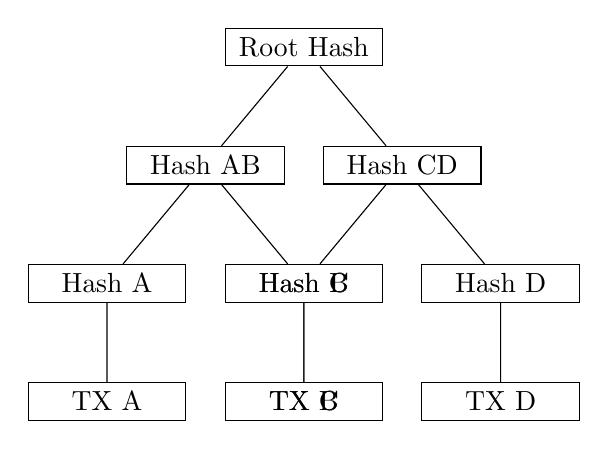
\begin{tikzpicture}[level distance=1.5cm, sibling distance=2.5cm, every node/.style={draw, rectangle, minimum width=2cm}]
        \node {Root Hash}
            child {node {Hash AB}
                child {node {Hash A}
                    child {node {TX A}}
                }
                child {node {Hash B}
                    child {node {TX B}}
                }
            }
            child {node {Hash CD}
                child {node {Hash C}
                    child {node {TX C}}
                }
                child {node {Hash D}
                    child {node {TX D}}
                }
            };
    \end{tikzpicture}
    \caption{Merkle Tree Structure}
\end{figure}

\textbf{Benefits:}

\begin{itemize}
    \item \keyword{Efficiency}: Quick verification without downloading all data
    \item \keyword{Security}: Any change detected immediately
    \item \keyword{Scalability}: Verification time stays constant
\end{itemize}

\textbf{Verification Process:}

\begin{figure}[H]
    \centering
    \begin{tikzpicture}[node distance=1.5cm, auto]
        \node [gtu state] (Tx) {Tx to Verify};
        \node [gtu block, right=of Tx] (Path) {Get Path};
        \node [gtu block, right=of Path] (Hash) {Hash Siblings};
        \node [gtu block, below=of Hash] (Root) {Compute Root};
        \node [draw, diamond, aspect=2, left=of Root] (Match) {Match Stored?};
        \node [gtu state, left=of Match] (Valid) {Valid};
        
        \draw [gtu arrow] (Tx) -- (Path);
        \draw [gtu arrow] (Path) -- (Hash);
        \draw [gtu arrow] (Hash) -- (Root);
        \draw [gtu arrow] (Root) -- (Match);
        \draw [gtu arrow] (Match) -- node[above] {Yes} (Valid);
    \end{tikzpicture}
    \caption{Merkle Verification Flow}
\end{figure}

\begin{mnemonicbox}
Merkle = Many Made One, Tree = Trustworthy
\end{mnemonicbox}

\orquestionmarks{4(a)}{3}{Discuss briefly about Hash pointer and how it is used in Merkle tree.}

\keyword{Hash Pointer Definition}: A data structure containing both the location of data and cryptographic hash of that data.

\begin{figure}[H]
    \centering
    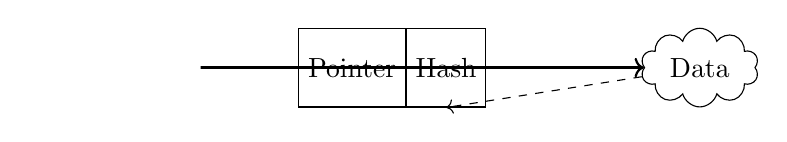
\begin{tikzpicture}[node distance=2cm, auto]
        \node [draw, rectangle, minimum height=1cm] (Ptr1) {Pointer};
        \node [draw, rectangle, minimum height=1cm, right=0pt of Ptr1] (Ptr2) {Hash};
        \node [draw, cloud, right=of Ptr2, aspect=2] (Data) {Data};
        \draw [->, thick] (Ptr1.west) to[out=180,in=180, looseness=2] (Data.west);
        \draw [->, dashed] (Data) -- (Ptr2.south);
    \end{tikzpicture}
    \caption{Hash Pointer Concept}
\end{figure}

\textbf{Usage in Merkle Tree:}

\begin{tabulary}{\linewidth}{L L}
    \toprule
    \textbf{Level} & \textbf{Hash Pointer Function} \\
    \midrule
    \textbf{Leaf Level} & Points to transaction, contains transaction hash \\
    \textbf{Internal Nodes} & Points to children, contains combined hash \\
    \textbf{Root} & Points to tree structure, contains overall hash \\
    \bottomrule
\end{tabulary}

\begin{itemize}
    \item \keyword{Verification}: Can detect any change in tree structure
    \item \keyword{Navigation}: Allows efficient traversal of tree
\end{itemize}

\begin{mnemonicbox}
Hash Pointer = Location + Verification
\end{mnemonicbox}

\orquestionmarks{4(b)}{4}{What is Hashing in Blockchain? How it is useful in Bitcoin?}

\keyword{Hashing Definition}: Mathematical function that converts input data into fixed-size string of characters.

\textbf{Bitcoin Usage:}

\begin{tabulary}{\linewidth}{L L}
    \toprule
    \textbf{Use Case} & \textbf{Purpose} \\
    \midrule
    \textbf{Block Linking} & Each block contains hash of previous block \\
    \textbf{Mining} & Find hash meeting difficulty requirement \\
    \textbf{Transaction IDs} & Unique identifier for each transaction \\
    \textbf{Merkle Root} & Summarize all transactions in block \\
    \bottomrule
\end{tabulary}

\begin{figure}[H]
    \centering
    \begin{tikzpicture}[node distance=2cm]
        \node [gtu block] (Input1) {Input Data};
        \node [gtu state, right=3cm of Input1] (Hash1) {Hash Output 1};
        \draw [gtu arrow, ->] (Input1) -- node[above] {SHA-256} (Hash1);
        
        \node [gtu block, below=of Input1] (Input2) {Input (Changed)};
        \node [gtu state, right=3cm of Input2] (Hash2) {Different Hash};
        \draw [gtu arrow, ->] (Input2) -- node[above] {SHA-256} (Hash2);
    \end{tikzpicture}
    \caption{Avalanche Effect in Hashing}
\end{figure}

\begin{mnemonicbox}
Hash = Fingerprint, Bitcoin = Built on Hashing
\end{mnemonicbox}

\orquestionmarks{4(c)}{7}{Explain classic Byzantine generals problem and Practical Byzantine Fault Tolerance in detail.}

\keyword{Byzantine Generals Problem}: A classic problem about achieving consensus in distributed systems with unreliable participants.

\begin{figure}[H]
    \centering
    \begin{tikzpicture}[node distance=2cm]
        \node [gtu block] (City) {City};
        \node [gtu state, above=of City] (G1) {General 1 (Honest)};
        \node [gtu state, left=of City, fill=red!10] (G2) {General 2 (Traitor)};
        \node [gtu state, right=of City] (G3) {General 3 (Honest)};
        
        \draw [->, thick] (G1) -- node[right] {Attack} (City);
        \draw [->, thick] (G3) -- node[left] {Attack} (City);
        
        \draw [->, dashed, thick, red] (G2) -- node[above, sloped] {Retreat} (G1);
        \draw [->, dashed, thick, red] (G2) -- node[above, sloped] {Attack} (G3);
    \end{tikzpicture}
    \caption{Byzantine Generals Traitor Scenario}
\end{figure}

\textbf{Practical Byzantine Fault Tolerance (pBFT):}

\begin{tabulary}{\linewidth}{L L L}
    \toprule
    \textbf{Phase} & \textbf{Action} & \textbf{Purpose} \\
    \midrule
    \textbf{Pre-prepare} & Leader broadcasts proposal & Initiate consensus round \\
    \textbf{Prepare} & Nodes validate & Ensure proposal is seen by all \\
    \textbf{Commit} & Nodes commit & Finalize consensus \\
    \bottomrule
\end{tabulary}

\begin{figure}[H]
    \centering
    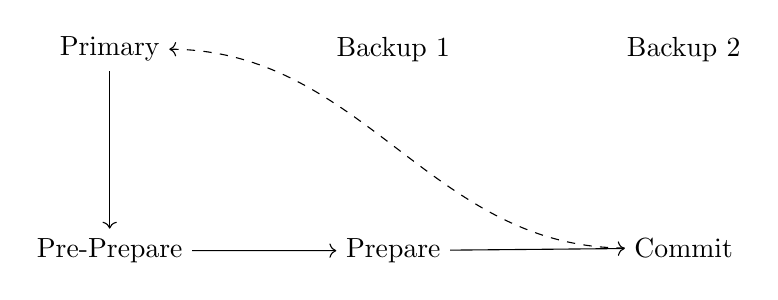
\begin{tikzpicture}[node distance=2cm]
        \node (P) {Primary};
        \node [right=of P] (B1) {Backup 1};
        \node [right=of B1] (B2) {Backup 2};
        
        \node [below=of P] (PP) {Pre-Prepare};
        \node [below=of B1] (Prep) {Prepare};
        \node [below=of B2] (Comm) {Commit};
        
        \draw [->] (P) -- (PP);
        \draw [->] (PP) -- (Prep);
        \draw [->] (Prep) -- (Comm);
        \draw [->, dashed] (Comm) to[out=180,in=0] (P);
    \end{tikzpicture}
    \caption{pBFT Consensus Phases}
\end{figure}

\begin{itemize}
    \item \keyword{Advantage}: Fast finality, good for permissioned networks
    \item \keyword{Limitation}: High communication overhead O(n squared)
\end{itemize}

\begin{mnemonicbox}
Byzantine = Bad actors, pBFT = Practical Fix
\end{mnemonicbox}

\questionmarks{5(a)}{3}{List and explain cryptocurrency wallets in blockchain.}

\textbf{Wallet Types:}

\begin{tabulary}{\linewidth}{L L}
    \toprule
    \textbf{Wallet Type} & \textbf{Description} \\
    \midrule
    \textbf{Hardware} & Physical device storing keys (High Security) \\
    \textbf{Software} & Application on computer/phone \\
    \textbf{Paper} & Keys printed on paper \\
    \textbf{Web} & Online wallet service \\
    \bottomrule
\end{tabulary}

\begin{figure}[H]
    \centering
    \begin{tikzpicture}[node distance=1.5cm, auto]
        \node [gtu block] (Wallet) {Wallet Interface};
        \node [gtu state, below left=of Wallet] (Keys) {Store Keys};
        \node [gtu state, below=of Wallet] (Sign) {Sign Tx};
        \node [gtu state, below right=of Wallet] (Bal) {Check Balance};
        
        \draw [gtu arrow] (Wallet) -- (Keys);
        \draw [gtu arrow] (Wallet) -- (Sign);
        \draw [gtu arrow] (Wallet) -- (Bal);
    \end{tikzpicture}
    \caption{Wallet Functions}
\end{figure}

\begin{mnemonicbox}
Wallet = Key Keeper, Not Coin Container
\end{mnemonicbox}

\questionmarks{5(b)}{4}{Write advantages and disadvantages of ERC-20 token.}

\keyword{ERC-20 Token Definition}: Standard protocol for creating tokens on Ethereum blockchain.

\begin{tabulary}{\linewidth}{L L L}
    \toprule
    \textbf{Aspect} & \textbf{Advantage} & \textbf{Disadvantage} \\
    \midrule
    \textbf{Standardization} & Work same way everywhere & Limited customization \\
    \textbf{Interoperability} & Compatible with wallets & - \\
    \textbf{Development} & Easy to create & Easy to create scams \\
    \textbf{Cost} & - & Gas fees can be high \\
    \bottomrule
\end{tabulary}

\begin{mnemonicbox}
ERC-20 = Easy and Expensive
\end{mnemonicbox}

\questionmarks{5(c)}{7}{What are dApps used for? Explain advantages and disadvantages of dApps.}

\keyword{dApps Definition}: Decentralized Applications that run on blockchain networks without central authority.

\textbf{Usage Categories:} DeFi, Gaming, Social Media, Marketplaces, Governance.

\begin{figure}[H]
    \centering
    \begin{tikzpicture}[node distance=1.5cm, auto]
        \node [gtu block] (Front) {Frontend (UI)};
        \node [gtu block, right=of Front] (Web3) {Web3 Lib};
        \node [gtu block, right=of Web3] (Contract) {Smart Contracts};
        \node [gtu block, below=of Contract] (Chain) {Blockchain};
        
        \draw [gtu arrow] (Front) -- (Web3);
        \draw [gtu arrow] (Web3) -- (Contract);
        \draw [gtu arrow] (Contract) -- (Chain);
    \end{tikzpicture}
    \caption{dApp Architecture}
\end{figure}

\textbf{Advantages vs Disadvantages:}

\begin{tabulary}{\linewidth}{L L}
    \toprule
    \textbf{Advantages} & \textbf{Disadvantages} \\
    \midrule
    Censorship Resistance & Poor User Experience \\
    Transparency & Scalability Issues \\
    No Downtime & High Costs (Gas) \\
    User Ownership & Technical Complexity \\
    \bottomrule
\end{tabulary}

\begin{mnemonicbox}
dApps = Decentralized but Difficult
\end{mnemonicbox}

\orquestionmarks{5(a)}{3}{Explain tokenized and token less Blockchain in detail.}

\begin{tabulary}{\linewidth}{L L L}
    \toprule
    \textbf{Aspect} & \textbf{Tokenized} & \textbf{Token-less} \\
    \midrule
    \textbf{Definition} & With native crypto & No native crypto \\
    \textbf{Purpose} & Incentive & Record keeping \\
    \textbf{Example} & Bitcoin, Ethereum & Hyperledger Fabric \\
    \textbf{Access} & Public (usually) & Private (Permissioned) \\
    \bottomrule
\end{tabulary}

\begin{figure}[H]
    \centering
    \begin{tikzpicture}[node distance=1.5cm]
        \node [gtu block] (Token) {Tokenized};
        \node [gtu state, below=of Token] (Incent) {Incentives};
        \node [gtu state, below=of Incent] (Miner) {Miners};
        
        \draw [gtu arrow] (Token) -- (Incent);
        \draw [gtu arrow] (Incent) -- (Miner);
        
        \node [gtu block, right=3cm of Token] (NoToken) {Token-less};
        \node [gtu state, below=of NoToken] (Perm) {Permissions};
        \node [gtu state, below=of Perm] (Auth) {Auth Nodes};
        
        \draw [gtu arrow] (NoToken) -- (Perm);
        \draw [gtu arrow] (Perm) -- (Auth);
    \end{tikzpicture}
    \caption{Incentive Models}
\end{figure}

\begin{mnemonicbox}
Token = Public Participation, Token-less = Private Permission
\end{mnemonicbox}

\orquestionmarks{5(b)}{4}{Write advantages and disadvantages of Hyperledger.}

\textbf{Advantages:}

\begin{itemize}
    \item \textbf{Enterprise Focus}: Designed for business use cases
    \item \textbf{Privacy}: Confidential transactions possible
    \item \textbf{Performance}: Higher transaction throughput
    \item \textbf{Permissioned}: Control who can participate
\end{itemize}

\textbf{Disadvantages:}

\begin{itemize}
    \item \textbf{Centralization}: Less decentralized than public blockchains
    \item \textbf{Complexity}: Requires technical expertise
    \item \textbf{No Token Economy}: Cannot leverage crypto incentives
\end{itemize}

\begin{mnemonicbox}
Hyperledger = High Performance, Low Publicity
\end{mnemonicbox}

\orquestionmarks{5(c)}{7}{Explain Smart contract. Write various applications of smart contract.}

\keyword{Smart Contract Definition}: Self-executing contracts with terms directly written into code, automatically enforced on blockchain.

\begin{figure}[H]
    \centering
    \begin{tikzpicture}[node distance=1.5cm, auto]
        \node [gtu block] (Create) {Create};
        \node [gtu block, right=of Create] (Deploy) {Deploy};
        \node [gtu block, right=of Deploy] (Monitor) {Monitor};
        \node [draw, diamond, aspect=2, below=of Monitor] (Cond) {Cond Met?};
        \node [gtu state, left=of Cond] (Exec) {Execute};
        
        \draw [gtu arrow] (Create) -- (Deploy);
        \draw [gtu arrow] (Deploy) -- (Monitor);
        \draw [gtu arrow] (Monitor) -- (Cond);
        \draw [gtu arrow] (Cond) -- node[above] {Yes} (Exec);
        \draw [gtu arrow] (Cond.east) -- ++(0.5,0) |- node[near start, right] {No} (Monitor);
    \end{tikzpicture}
    \caption{Smart Contract Workflow}
\end{figure}

\textbf{Applications:}

\begin{tabulary}{\linewidth}{L L}
    \toprule
    \textbf{Industry} & \textbf{Application} \\
    \midrule
    \textbf{Finance} & Automated loans (DeFi) \\
    \textbf{Real Estate} & Property transfers without agents \\
    \textbf{Supply Chain} & Automated tracking and payments \\
    \textbf{Insurance} & Automatic claim payouts \\
    \bottomrule
\end{tabulary}

\begin{mnemonicbox}
Smart Contract = Self-executing, Solves Problems
\end{mnemonicbox}

\end{document}

